\documentclass[portrait]{usydposter}
\usepackage{xspace}
\usepackage{graphicx}

\newcommand{\acronym}[1]{\textsc{#1}\xspace}
\newcommand{\cf}[1]{\mbox{$\it{#1}$}}
\newcommand{\todo}[1]{{\color{red} #1}}

\newcommand{\ngram}{n-gram\xspace}
\newcommand{\ngrams}{{\ngram}s\xspace}
\newcommand{\candc}{C\&C\xspace}
\newcommand{\ccgbank}{CCGBank\xspace}
\newcommand{\ccg}{\acronym{ccg}}
\newcommand{\cky}{\acronym{cky}}
\newcommand{\nlp}{\acronym{nlp}}
\newcommand{\np}{\acronym{np}}
\newcommand{\pos}{\acronym{pos}}
\newcommand{\wsj}{\acronym{wsj}}

\newcommand{\los}{\acronym{los}}
\newcommand{\roc}{\acronym{roc}}
\newcommand{\auc}{\acronym{auc}}
\newcommand{\nn}{\acronym{nn}}
\newcommand{\cfs}{\acronym{cfs}}

\DeclareGraphicsExtensions{.png}

\flushbottom

\title{Improved Prediction of Hospital Length of Stay for Severe Injury}
\author{Tianyu Pu \xspace \texttt{tianyu.pu@sydney.edu.au}}

\begin{document}

\makeheader

\begin{multicols}{3}

% =============================================================================
\section{Problem}
\noindent There are limited beds in hospital trauma wards, and yet there is a
constant demand for these beds by the inflow of severely injured patients. Many
patients are initially allocated to these beds when they could be better
treated in another specialised ward.
\begin{center}
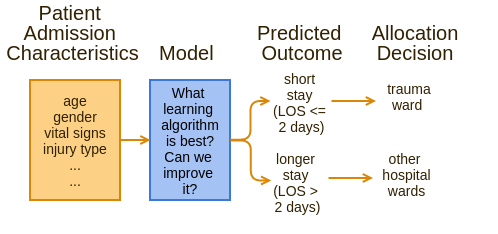
\includegraphics[scale=0.75]{problem-diag}
\end{center}
\noindent If we could accurately classify patients with hospital length of
stay (\los) of 2 days or less versus those who require longer stays, we could
make a more informed decision whether or not to place them in another ward
when they are admitted, rather than wasting time and resources
transferring them to another ward later.

% =============================================================================
\section{Motivation}
\noindent Accurate prediction of the \los in various medical
domains (such as burns) has been extensively studied
as it is a key indicator of how hospitals use their limited resources.
The current literature focuses extensively
on generalised linear models, with some applications
of techniques from machine learning such as neural networks.
There has been no work done in systematically
applying a range of machine learning techniques to \los prediction, and
specifically not to the trauma medical domain.
Additionally, there has been little work done in feature
transformation and selection when \los prediction models are created.

% =============================================================================
\section{Contribution}
\noindent We systematically investigate feature transformation and selection
techniques in the construction of a \los prediction model for trauma patients.
We also apply and evaluate a comprehensive range of
classification algorithms on data from the trauma domain as well as from a
general hospital setting.

In addition, we
propose a new nearest-neighbour (\nn) algorithm, ranked \nn, which takes
into account the
predictive relevance of features when computing the distance to the nearest
neighbours.

% =============================================================================
\section{Datasets}
\noindent Our study was conducted on two datasets: one with 2546 records from
the Trauma Services Centre at the Royal Prince Alfred Hospital in Sydney,
consisting of
trauma patients admitted to the centre between 2007--11;
the other from the Hospital das
Foras Armadas in Portugal with 17546 records collected from 2000--13 and
covering a wide range of medical diagnoses.

% =============================================================================
\section{Approach}
\subsection{Feature preprocessing and investigation of learning algorithms}
\begin{center}
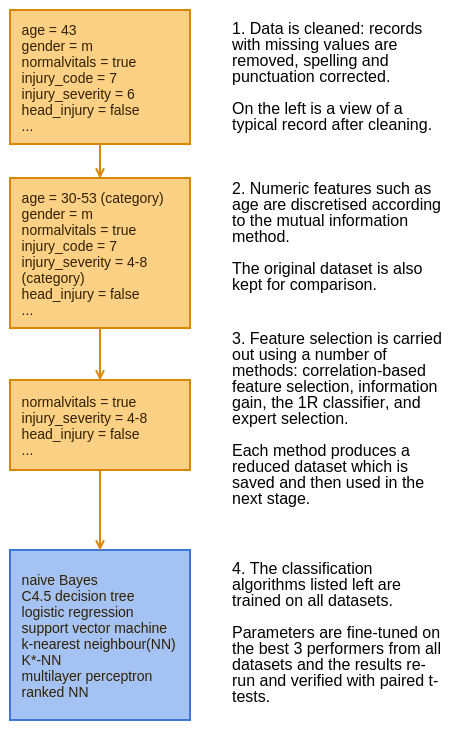
\includegraphics[scale=0.75]{approach}
\end{center}

\subsection{Ranked nearest neighbour}
\noindent \textit{Idea: the contribution of a feature to the distance between
two records should be proportional to its level of `relevance' or predictive
power with respect to the outcome variable, \los.} This is how it works:
\begin{center}
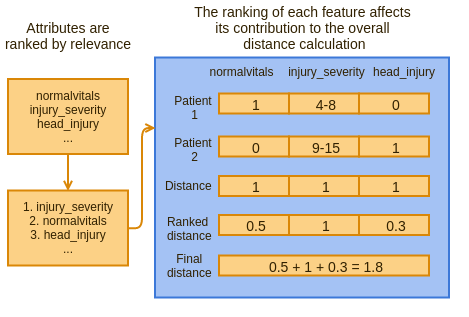
\includegraphics[scale=0.75]{ranked-nn}
\end{center}

% =============================================================================
\section{Evaluation Metrics}
\noindent \textit{Area under the receiver-operating characteristic curve (\auc)},
the extent to which the classification algorithm is able to distinguish between
patients that require a stay of less than 2 days or those who require longer.
Randomly picking between two outcomes has \auc 0.5; the maximum is 1,
indicating perfect discriminating ability.

Our \textit{baseline} is the logistic regression model derived in
\cite{Dinh2013a}, as we aim to improve upon the results they achieved for
trauma patients.
All \auc figures are obtained from
\textit{10-fold stratified cross-validation}.

% =============================================================================
\section{Results}
\subsection{Trauma dataset}
Discretisation significantly improved the performance of all classifiers,
regardless of feature selection method. Feature selection usually improved
performance but depended on the method, with \cfs the most effective. Ranked
\nn is not affected by discretisation and does not require feature selection,
and improves upon baseline \auc by 1-2\% (0.82-0.83)
while being faster to train than more sophisticated methods.
The best classifiers were logistic regression
and SVM with discretisation with mean \auc 0.84 (baseline 0.81).
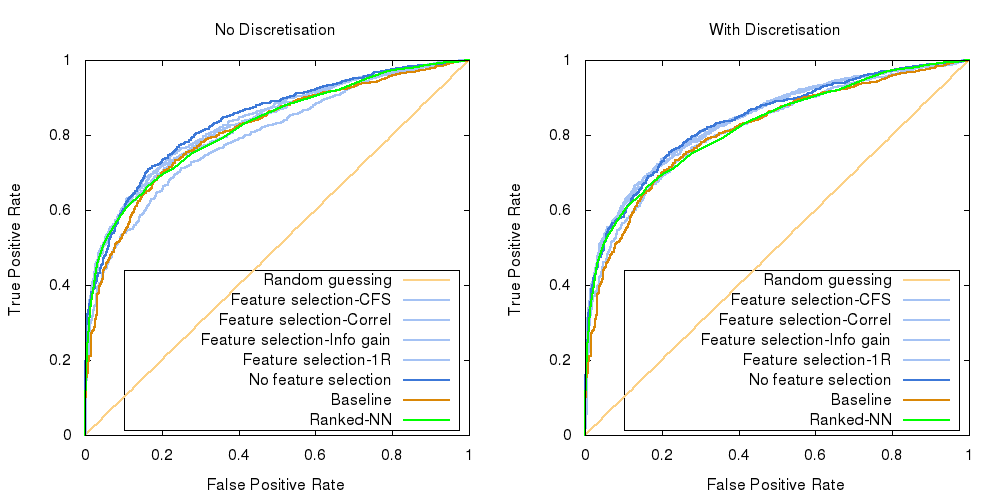
\includegraphics[scale=0.53]{trauma}

\subsection{General dataset}
All classification algorithms performed very well regardless of discretisation
or feature selection as the original features were very good at predicting
\los. Again, performing discretisation makes the method of feature selection
less important, as it stabilises performance overall. The best results were
mean \auc 0.994 with logistic regression and SVM regardless of discretisation;
ranked \nn had mean \auc 0.992 with less training time.
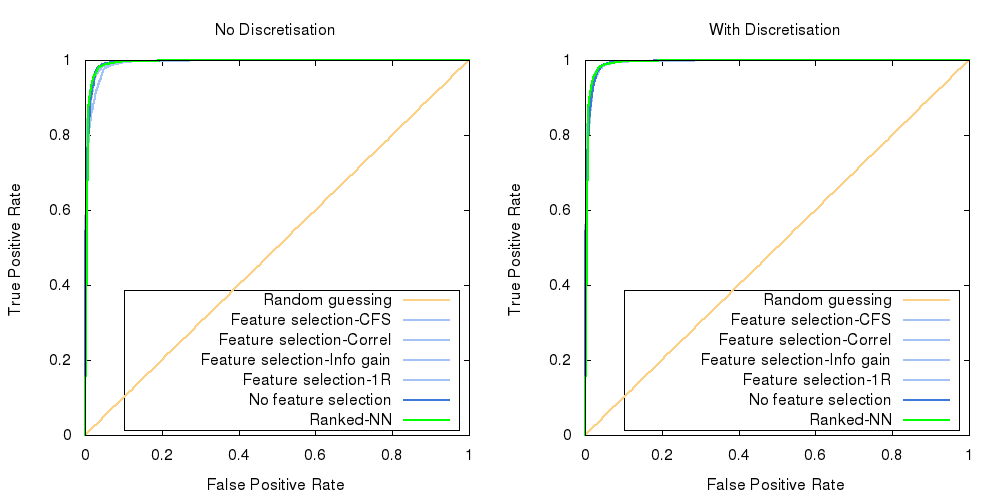
\includegraphics[scale=0.53]{portugal}

% =============================================================================
\section{Conclusions and Future Work}
\noindent Careful application of discretisation and feature selection can
improve the predictive power of classification algorithms. We proposed a
general method to improve the \los predictions for a trauma and general
hospital domain, and showed overall improvements in \auc from 2-4\% from the
baseline. This general method will be a useful starting point for those
investigating \los prediction.

Furthermore, ranked \nn performs 1-2\% better than the baseline, is
moderately fast to train, and is not strongly affected by discretisation and
irrelevant features.

There is
room to further evaluate this method in other medical areas, as well as
implementation of such a model as a decision support tool for physicians.
Additionally, improving upon the ranked \nn algorithm to account for different
methods of weighting features and calculating ranks can also be investigated.

% =============================================================================
\section{Acknowledgements}
\noindent
Many thanks to Dr Michael Dinh, co-director of Royal Prince Alfred
Hospital Trauma Services, for providing the trauma data and medical domain
guidance; and thanks also to Associate Professor Paulo Cortez, from the
Department of Information Systems at the University of
Minho in Portugal, for providing an extensive general \los dataset.

% =============================================================================

\references
\bibliography{../thesis/references}

\end{multicols}
\end{document}
